\section{La form di richiesta}
L'interfaccia utente è basilare, la form di richiesta permette all'utente di inserire i vertici dell'area di partenza. Nel corso dello sviluppo del mio progetto ho utilizzato come punti di riferimento le coordinate di Parigi e Madrid.

\begin{figure}[H]
	\centering
	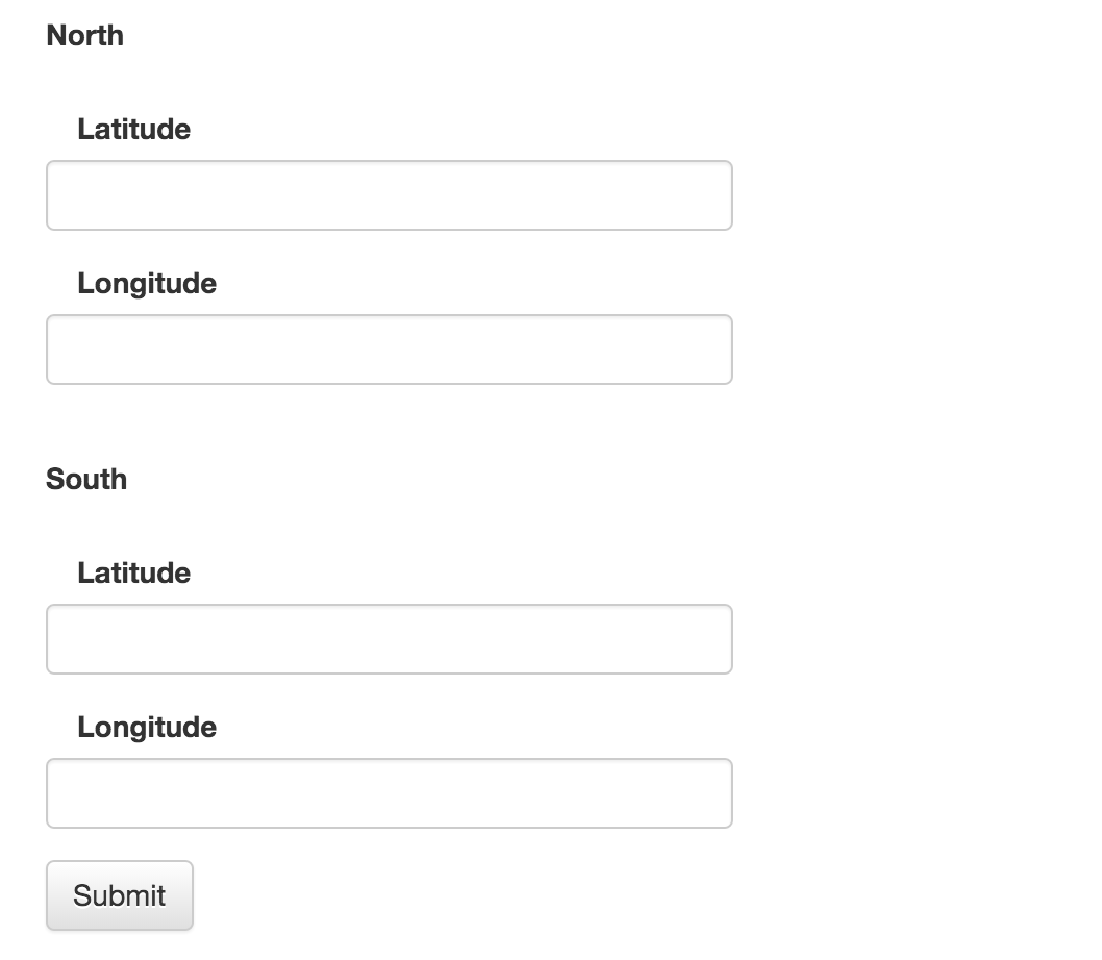
\includegraphics[scale=0.5]{figure/formexample.eps}
	\caption{Struttura della form per la richiesta dell'area iniziale}
\end{figure}

\begin{figure}[H]
	\centering
	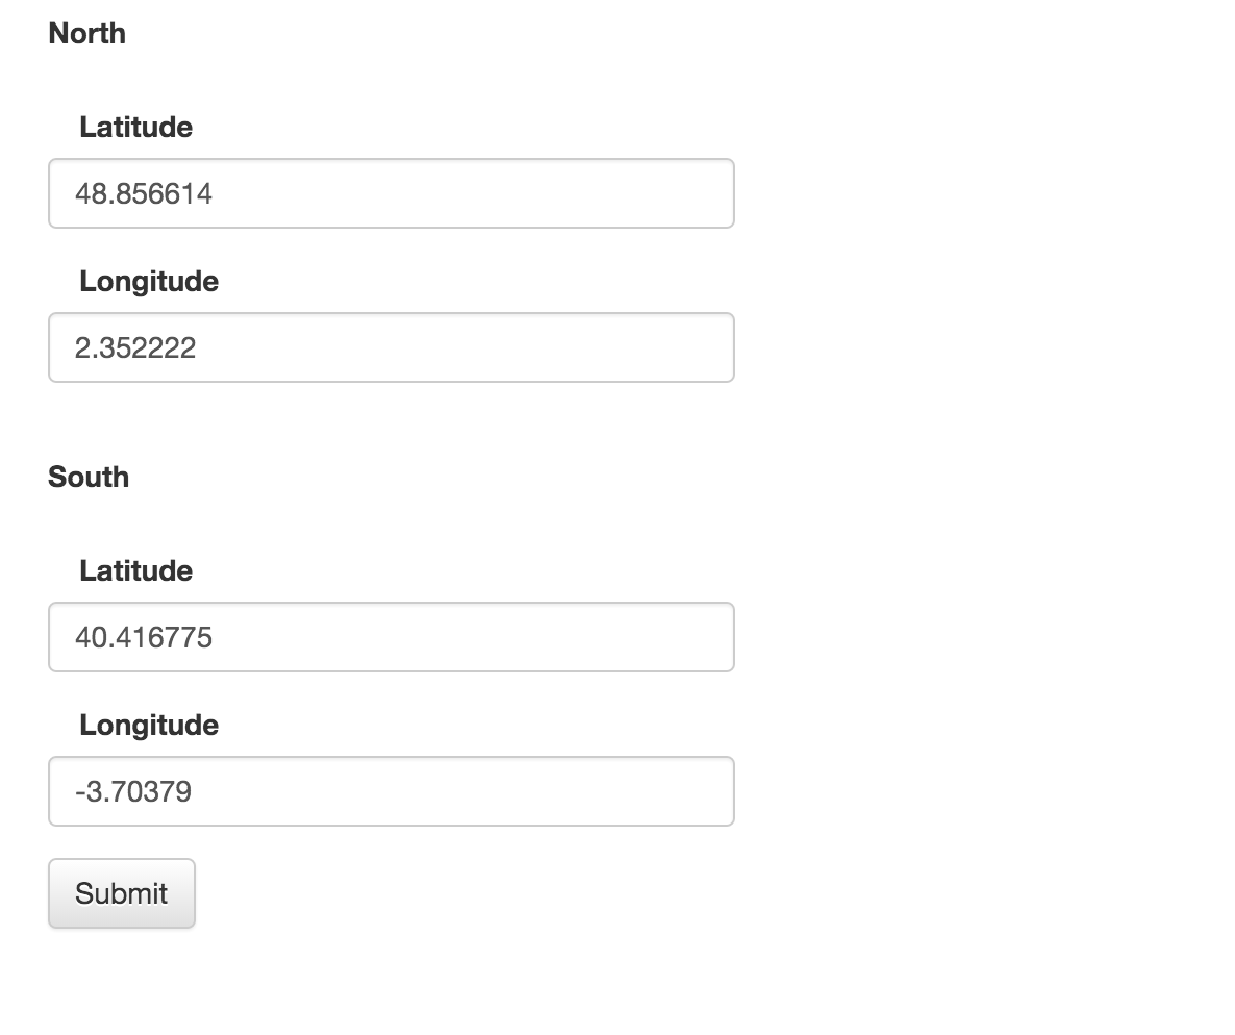
\includegraphics[scale=0.5]{figure/formexample_1.eps}
	\caption{Inserimento delle coordinate di Parigi e Madrid}
\end{figure}

\section{La proiezione su un piano prospettico}
Una volta inserite le coordinate dei due punti e inviate le informazioni al server cliccando il tasto "Submit", l'utente sarà reindirizzato sulla pagina contenente la nostra canvas 3D. A questo punto la mappa verrà caricata sulla scena e visualizzata in chiave prospettica.

\begin{figure}[H]
	\centering
	\includegraphics[scale=0.4]{figure/scenainiziale.eps}
	\caption{Proiezione dell'area tra Parigi (in alto a destra) e Madrid (in basso a sinistra)}
\end{figure}

\begin{figure}[H]
	\centering
	\includegraphics[width=\textwidth]{figure/romanapoli.eps}
	\caption{Proiezione dell'area tra Roma (in alto a sinistra) e Napoli (in basso a destra)}
\end{figure}

Una volta caricata la cartina dell'area desiderata sarà possibile iniziare ad interagire con l'ambiente creato e dunque iniziare la navigazione della mappa.

\begin{figure}[H]
	\centering
	\includegraphics[width=\textwidth]{figure/spostamento.eps}
	\caption{Questa è la situazione dopo una serie di spostamenti}
\end{figure}

L'utilizzatore non si accorgerà del caricamento di una nuova tile, se non per la presenza del logo gi \textit{Google} e la dicitura dei Termini e condizioni di utilizzo, presenti in basso a ogni tile.

\begin{figure}[H]
	\centering
	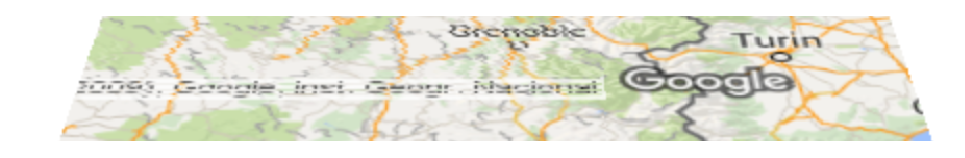
\includegraphics[width=\textwidth]{figure/terminiecondizioni.eps}
	\caption{La scritta delle condizioni di utilizzo e il logo di Google stampati sulla mappa}
\end{figure}

Nel momento in cui si volesse effettuare lo zoom, basterà premere il tasto W per aumentare il dettaglio o S per diminuirlo.

\begin{figure}[H]
	\centering
	\includegraphics[width=0.5\textwidth]{figure/zoomin.eps}
	\caption{Risultato dell'azione di zoom in sulla mappa}
\end{figure}

\begin{figure}[H]
	\centering
	\includegraphics[width=0.5\textwidth]{figure/zoomout.eps}
	\caption{Risultato dell'azione di zoom out sulla mappa}
\end{figure}

Una volta ottenuto il risultato dello zoom sarà possibile riprendere con la navigazione e spostarsi lungo tutta la terra.

\begin{figure}[H]
	\centering
	\includegraphics[width=\textwidth]{figure/spostamento2.eps}
	\caption{Nuovo esempio di spostamento}
\end{figure}